\section{SpecBraM}\label{sec:method}
\begin{figure*}[t]\centering
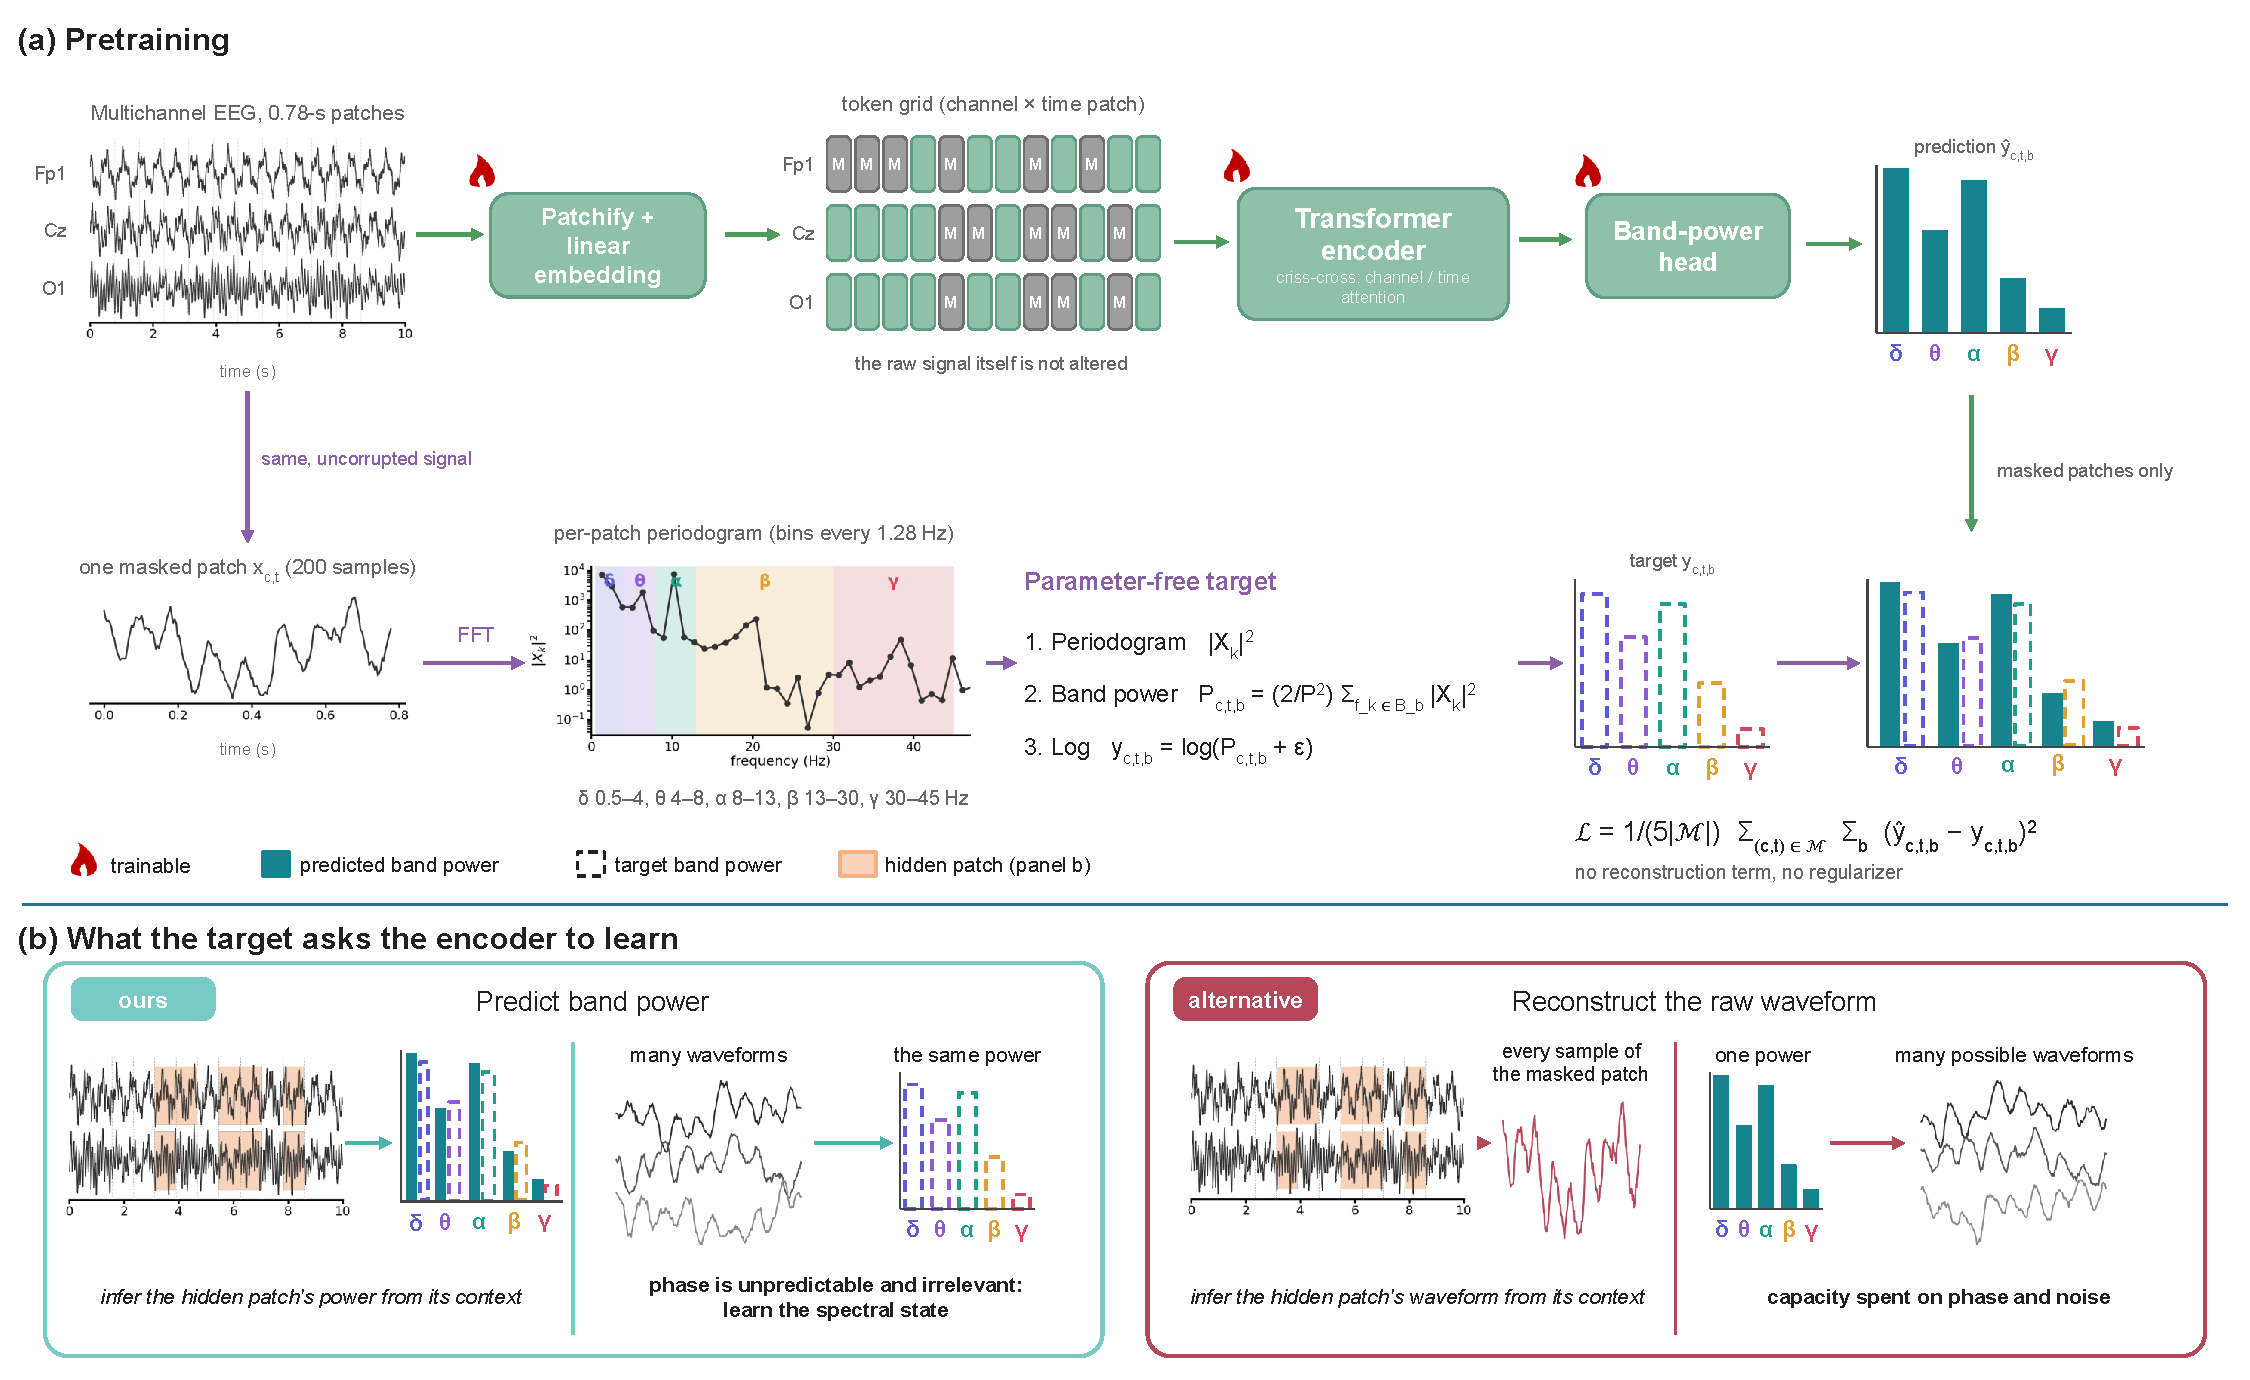
\includegraphics[width=\textwidth]{figures/pipeline_v2.pdf}
\caption{\textbf{SpecBraM pretraining.} (a) Each channel is cut into 0.78-s patches that are
embedded linearly; 30\% of the (channel, time) tokens are replaced by a learnable [M] token,
while the signal itself is not altered. A criss-cross transformer encodes the token grid and a
linear head predicts five log band powers for every masked token. The target is computed from
the periodogram of the uncorrupted patch and has no parameters. (b) Predicting band power asks
the encoder to infer the spectral state of a hidden patch from its context; reconstructing the
waveform also asks for sample-level details, including phase, that the context may only
partly determine.}
\label{fig:pipeline}
\end{figure*}
\noindent\textbf{Input and tokens.} A 10-s window at 256\,Hz over the 19 channels of the
10--20 montage, normalized per recording (median and interquartile range), is cut per channel
into non-overlapping patches of $P{=}200$ samples ($0.78$\,s), giving a token grid with
$C{=}19$ channels and $T_p{=}\lfloor 2560/200\rfloor{=}12$ time patches; the last 160 samples
($0.625$\,s) of each window are not used, during pretraining and in every downstream window
(including each of the three 10-s windows of a 30-s sleep epoch; 5-s TUEV windows give six
patches). The main model embeds each patch with a single
linear map (as CBraMod does). A variant decomposes each patch with a learnable 5-band
filterbank before embedding (``filterbank tokenizer''); we report both because the target
study crosses tokenizer and target.

\noindent\textbf{Encoder and masking.} A 12-layer criss-cross transformer ($D{=}512$, 8 heads;
51.3M parameters) alternates attention along the channel and time axes, with learned channel
and time position embeddings. Each (channel, time) patch is masked independently with
probability $0.3$; the embeddings of masked patches are replaced by a learned mask token.

\noindent\textbf{Target.} For each patch $\bm{x}_{c,t}\in\mathbb{R}^{P}$ of the uncorrupted
signal, let $X_k=\sum_{\tau}x_{c,t,\tau}e^{-i2\pi k\tau/P}$ be its discrete Fourier transform
(rectangular window, no padding) at $f_k=kf_s/P$. For the five classical bands
$B_1,\dots,B_5=[0.5,4),[4,8),[8,13),[13,30),[30,45)$\,Hz
($\delta,\theta,\alpha,\beta,\gamma$),
\begin{align}
P_{c,t,b}&=\frac{2}{P^2}\sum_{f_k\in B_b}|X_k|^2,\nonumber\\
y_{c,t,b}&=\log\bigl(P_{c,t,b}+\varepsilon\bigr),\qquad b=1,\dots,5, \label{eq:target}
\end{align}
with $\varepsilon=10^{-3}$ in the robust-scaled input units; its effect depends on the band
power relative to this floor. By one-sided Parseval, $P_{c,t,b}$ is the variance of
the patch within band $b$; it equals the band-averaged periodogram of Sec.~\ref{sec:theory}
times the per-band constant $2m_b/P$, where $m_b$ is the number of Fourier bins in the band
(3/3/4/13/12 at $\Delta f=1.28$\,Hz; Table~\ref{tab:bins}). The target is fixed (no learnable
parameters) and patch-local: it uses no samples of neighbouring, possibly visible patches.

\noindent\textbf{Choice of bands.} The classical partition reflects physiologically distinct
rhythms (slow-wave activity, theta, the posterior alpha rhythm and sleep spindles at its upper
edge, beta and gamma) and is the vocabulary in which sleep scoring and clinical EEG reports are
written. Its exact edges are conventions (alpha is given as 8--12 or 8--13\,Hz, and individual
alpha frequency varies by several hertz), so we treat them as a sensible default rather than
an optimum.

\noindent\textbf{Objective.} A linear head maps each encoder output $H_{c,t}$ to five
predictions $\hat y_{c,t,b}$. With $\mathcal{M}$ the set of masked patches,
\begin{equation}
\mathcal{L}=\frac{1}{5|\mathcal{M}|}\sum_{(c,t)\in\mathcal{M}}\sum_{b=1}^{5}
\bigl(\hat y_{c,t,b}-y_{c,t,b}\bigr)^2,
\label{eq:loss}
\end{equation}
the mean squared error over the masked patches and the five bands. There is no
reconstruction term, no latent-prediction term and no regularizer. The target is fixed;
this alone does not guarantee a noncollapsed representation. The waveform-reconstruction controls replace the loss of
Eq.~\eqref{eq:loss} by the MSE between a linear decoder output and the raw samples of each
masked patch (``raw'') or five band-pass-filtered versions of the patch waveform (fixed 65-tap
Hann-windowed cosine filters centred at 2/6/10/21/38\,Hz; ``band-waveform''), with everything
else unchanged.
